\chapter{Конструкторский раздел}
    \section{IDEF0}
        На рисунках \ref{idef0:A0} - \ref{idef0:A1} показаны
        нулевой и первый уровень диаграммы IDEF0, показывающие процесс
        мониторинга системных вызовов.
         
    \begin{figure}[h!]
        \centering
        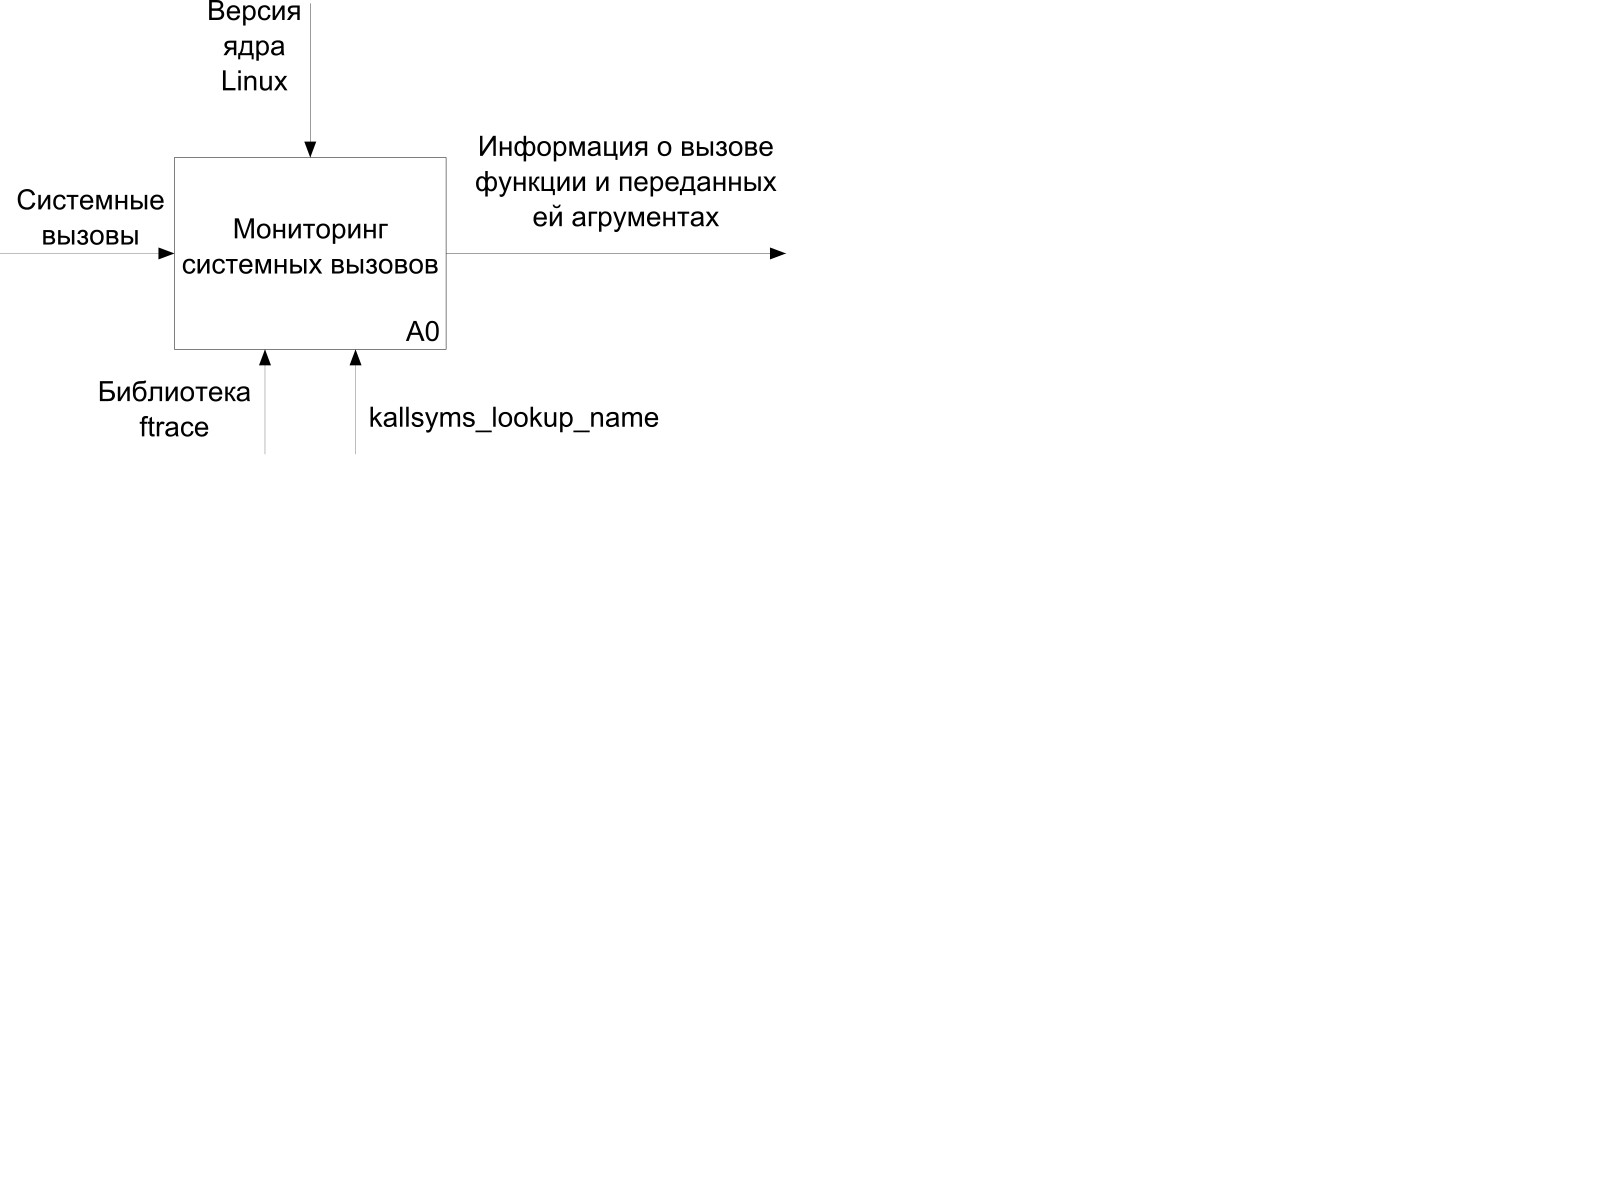
\includegraphics[width = 0.7 \textwidth]{diagrams/src/idef0_A0.pdf}
        \caption{IDEF0 нулевого уровня.}
        \label{idef0:A0}
    \end{figure}

    \begin{figure}[h!]
        \centering
        \includegraphics[width = 0.7 \textwidth]{diagrams/src/idef0_A1.pdf}
        \caption{IDEF0 первого уровня.}
        \label{idef0:A1}
    \end{figure}

        В состав программного обеспечения входит один загружаемый модуль ядра, 
        который следит за вызовом определенных функций, 
        с последующим логированием информации
        об аргументах и имени вызываемой функции в системный журнал (/var/log/syslog).

    \section{Используемые структуры данных}
        В новых версиях ядра прототип обработчика системного вызова описывается следующим образом (листинг \ref{lst:syscall-hooking:signature}):
        \begin{lstlisting}[language=C, label=lst:syscall-hooking:signature, title=Прототип обработчиков системных вызовов]
typedef asmlinkage long ( *syscall_t)(const struct pt_regs *);
    \end{lstlisting}
        где struct pt\_regs -- структура, описывающая 
        регистры процессора, которая может отличаться для разных версий ядра и процессоров.
        В документации ядра Linux описано назначения регистров для каждого конкретного системного вызова \cite{linux-syscall-reference}.
        Одно из определений struct pt\_regs представлено в листинге \ref{lst:syscall-hooking:pt_regs} \cite{linux-pt_regs}.

    \begin{lstlisting}[language=C, label=lst:syscall-hooking:pt_regs, title=Структура регистров]
struct pt_regs {
    /*
        * NB: 32-bit x86 CPUs are inconsistent as what happens in the
        * following cases (where %seg represents a segment register):
        *
        * - pushl %seg: some do a 16-bit write and leave the high
        *   bits alone
        * - movl %seg, [mem]: some do a 16-bit write despite the movl
        * - IDT entry: some (e.g. 486) will leave the high bits of CS
        *   and (if applicable) SS undefined.
        *
        * Fortunately, x86-32 doesn't read the high bits on POP or IRET,
        * so we can just treat all of the segment registers as 16-bit
        * values.
        */
    unsigned long bx;
    unsigned long cx;
    unsigned long dx;
    unsigned long si;
    unsigned long di;
    unsigned long bp;
    unsigned long ax;
    unsigned short ds;
    unsigned short __dsh;
    unsigned short es;
    unsigned short __esh;
    unsigned short fs;
    unsigned short __fsh;
    /* On interrupt, gs and __gsh store the vector number. */
    unsigned short gs;
    unsigned short __gsh;
    /* On interrupt, this is the error code. */
    unsigned long orig_ax;
    unsigned long ip;
    unsigned short cs;
    unsigned short __csh;
    unsigned long flags;
    unsigned long sp;
    unsigned short ss;
    unsigned short __ssh;
};
    \end{lstlisting}

        Ключевой структурой, используемой ftrace для установки перехвата функции,
        является struct ftrace\_ops, которая описывает каждую перехватываемую функцию
        (листинг \ref{lst:ftrace-hooking:struct:ftrace_ops}) \cite{linux-ftrace_ops}.
        Обязательной для заполнения является поле func -- адрес функции обратного вызова,
        которая будет вызываться в самом начале перехватываемой функции.
        Для решения проблемы рекурсии (перехватываемая функция вызывает коллбэк-функцию, которая опять вызывает перехватываемую)
        используют вспомогательную структуру struct ftrace\_hook (листинг \ref{lst:ftrace-hooking:struct}), в которой описывается
        имя перехватываемой функции, 
        адрес функции-перехватчика,
        адрес перехватываемой функции и
        struct ftrace\_ops.

    \begin{lstlisting}[language=C, label=lst:ftrace-hooking:struct:ftrace_ops, title=struct ftrace\_ops]
typedef void ( *ftrace_func_t)(unsigned long ip, unsigned long parent_ip,
        struct ftrace_ops *op, struct pt_regs *regs);

struct ftrace_ops {
    ftrace_func_t			func;
    struct ftrace_ops __rcu		*next;
    unsigned long			flags;
    void				*private;
    ftrace_func_t			saved_func;
#ifdef CONFIG_DYNAMIC_FTRACE
    struct ftrace_ops_hash		local_hash;
    struct ftrace_ops_hash		*func_hash;
    struct ftrace_ops_hash		old_hash;
    unsigned long			trampoline;
    unsigned long			trampoline_size;
    struct list_head		list;
#endif
};
    \end{lstlisting}

    \begin{lstlisting}[language=C, label=lst:ftrace-hooking:struct, title=struct ftrace\_hook]
struct ftrace_hook {
    const char *name;
    void *function;
    void *original;

    unsigned long address;
    struct ftrace_ops ops;
};
    \end{lstlisting}

    \section{Алгоритм внедрения функции-перехватчика в таблицу системных вызовов}
        \label{design:alg:hook:syscall_table}
        Алгоритм встраивания функций-перехватчиков в таблицу
        системных вызовов представлен на рисунке \ref{schema:syscall:init:hook:alg}.
        \begin{figure}[h!]
            \centering
            \includegraphics[width = 0.5 \textwidth]{alg-init-syscall-table.pdf}
            \caption{Схема алгоритма встраивания функций-перехватчиков в таблицу системных вызовов.}
            \label{schema:syscall:init:hook:alg}
        \end{figure}

        Для поиска адреса системной таблицы используется функция kallsyms\_lookup\_name,
        которая позволяет найти абсолютный адрес любого экспортируемого символа ядра.
        Номера системных вызовов описаны в исходном коде линукса \cite{linux-nomer-syscall}.
        Зная их и начальный адрес таблицы, можно получить и запомнить абсолютные адреса оригинальных системных вызовов.
        Однако таблица системных вызовов находиться в области памяти доступной только на чтение,
        поэтому на время изменения адрес обработчика системного вызова 
        требуется отключить глобальную защиту страниц от записи,
        изменением флага WP (Write Protection) в регистре CR0.

        Восстановление системных вызовов происходит аналогично перехвату,
        только в таблицу записываются изначальные адреса обработчиков.

    \section{Алгоритм перехвата функций с использованием библиотеки ftrace}
        \label{design:alg:hook:ftrace}
        Алгоритм встраивания функций-перехватчиков в функции ядра, 
        используя ftrace, представлен на рисунке \ref{schema:ftrace:init:hook:alg}.
        \begin{figure}[h!]
            \centering
            \includegraphics{alg-ftrace-init.pdf}
            \caption{Схема алгоритма встраивания функций-перехватчиков, используя ftrace.}
            \label{schema:ftrace:init:hook:alg}
        \end{figure}

        Для перехвата функции ядра с помощью ftrace необходимо сначала найти и сохранить её адрес.
        Аналогично поиску адреса системной таблицы для этого можно использовать функцию kallsyms\_lookup\_name.
        После чего устанавливается функция обратного вызова и необходимые флаги ftrace,
        включается обработка ftrace при вызове перехватываемой функции
        и регистрируется перехватчик.

        Отключение перехвата происходит в обратном порядке:
        дерегистрация перехвата ftrace, потом отключение ftrace для функции.


%         \begin{lstlisting}[language=C, label=lst:ftrace-hooking:macro, caption=Макрос для заполнения структуры перехватываемой функции]
% #define HOOK(_name, _hook, _orig)   \
% {                            \
%     .name = (_name),         \
%     .function = (_hook),     \
%     .original = (_orig),     \
% }

% /* массив перехватываемых функций */
% static struct ftrace_hook hooks[] = {
%     HOOK(<func name>, <hook func>, <original func>)
% };
%         \end{lstlisting}

%     \begin{lstlisting}[language=C, label=lst:ftrace-hooking:resolve_hook_address, caption=Поиск адреса функции по символьному имени]
% /* ftrace.h */
% #define MCOUNT_INSN_SIZE	4 /* sizeof mcount call */

% #define USE_FENTRY_OFFSET 0
% #if !USE_FENTRY_OFFSET
% #pragma GCC optimize("-fno-optimize-sibling-calls")
% #endif

% static int fh_resolve_hook_address(struct ftrace_hook *hook)
% {
%     hook->address = kallsyms_lookup_name(hook->name);

%     if (!hook->address)
%     {
%         printk(KERN_DEBUG "unresolved symbol: %s\n", hook->name);
%         return -ENOENT;
%     }

% #if USE_FENTRY_OFFSET
%     *((unsigned long*) hook->original) = hook->address + MCOUNT_INSN_SIZE;
% #else
%     *((unsigned long*) hook->original) = hook->address;
% #endif
%     return 0;
% }
%     \end{lstlisting}

    Для решения проблемы рекурсии используется алгоритм представленный на рисунке \ref{schema:ftrace:hook:alg}.
    В начале каждой функции ядра, для которой включён ftrace,
    находиться вызов функции \_\_fentry\_\_(),
    который вызывает функцию защиты от рекурсии,
    анализирующая значение parent\_ip -- адрес вызывающей стороны,
    на основании которого
    принимается решение о необходимости вызова функции перехватчика.
    Однако для корректного изменения регистра ip необходимо установить соответствующие флаги
    при регистрации обработчика:
    \begin{enumerate}
        \item FTRACE\_OPS\_FL\_IP\_MODIFY информирует ftrace, что регистр rip может быть изменён;
        \item FTRACE\_OPS\_FL\_SAVE\_REGS передавать struct pt\_regs исходного системного вызова хуку 
            (необходим для установки FTRACE\_OPS\_FL\_IP\_MODIFY);
        \item FTRACE\_OPS\_FL\_RECURSION\_SAFE отключает встроенную защиту от рекурсий.
    \end{enumerate}

    \begin{figure}[h!]
        \centering
        \includegraphics{alg-ftrace-hook.pdf}
        \caption{Схема алгоритма защиты от рекурсии.}
        \label{schema:ftrace:hook:alg}
    \end{figure}

    % Недостатком ftrace является возможность бесконечной рекурсии при перехвате функции,
    % в результате чего может произойти паника системы.
    % Существуют два способа избежать этого:
    % \begin{enumerate}
    %     \item обнаружить рекурсию, посмотрев на адрес возврата функции;
    %     \item перепрыгнуть через вызов ftrace (+ MCOUNT\_INSN\_SIZE).
    % \end{enumerate}
    % Для переключения между этими методами существует флаг USE\_FENTRY\_OFFSET.
    % Если установлено значение 0, используется первый вариант, в противном случае -- второй.

    % Если используется первый вариант, то необходимо отключить защиту, которую предоставляет ftrace.
    % Она работает на сохранение регистров возврата rip, но он будет изменён нами,
    % поэтому следует реализовать собственные средства защиты.
    % Все сводится к тому, что в .original поле ftrace\_hook структуры 
    % устанавливается адрес памяти системного вызова, указанного в .name.
    % Для корректной работы необходимо указать следующие флаги:

    Алгоритм работы всех функций-перехватчиков данных системных вызовов
    одинаков: логируется вызовы конкретного обработчика и передаваемые ему аргументы,
    после чего вызывается оригинальная функции, результат которой возвращается вызывающей стороне.
    Схема алгоритма функции-перехватчика представлена на рисунке \ref{schema:syscall:hook:alg}.

    \begin{figure}[h!]
        \centering
        \includegraphics{alg-syscall-table-hook.pdf}
        \caption{Схема алгоритма работы <<перехватчика>>.}
        \label{schema:syscall:hook:alg}
    \end{figure}

% \section{Связь структур}
%     Получение по файловому дескриптору имени файла.
%     % current->files->fdt->fd[fd]->f_path.dentry->d_iname

% \section{Вывод}
%     В данном разделе была рассмотрена общая архитектура приложения и
%     методы перехвата функций с помощью таблицы системных вызовов и ftrace.

\pagebreak